\section{Misura utilizzata}
Per misurare l'errore relativo abbiamo utilizzato la formula fornita dalla traccia:
$$\textrm{errore relativo } = \frac{||x - xe||_2}{||xe||_2}$$
dove, dati $A \in \mathbb{R}^{n \times n}$ e $xe \in \mathbb{R}^n$ con $xe = [1, 1, 1, \dots, 1]$, 
calcoliamo il termine noto del sistema $Ax = b$ come $b = A \cdot xe$. 
Il vettore $x$ è ottenuto risolvendo il sistema di equazioni $Ax = b$.
La risoluzione del sistema in C++ e in Matlab è già stata mostrata rispettivamente ai listings \ref{lst:execution-time-cpp} e \ref{lst:execution-time-matlab}.
\section{Analisi dei risultati}
Le misurazioni ottenute per entrambi i programmi su piattaforma Windows e su Linux sono riportate rispettivamente in figura \ref{fig:windows_relerr} 
e \ref{fig:linux_relerr}. Il confronto delle misurazioni ottenute per tutti i sistemi operativi è invece riportato in figura \ref{fig:complete_relerr}. Come si può evincere
dai grafici, la misura dell'errore relativo non dipende dal sistema operativo su cui si eseguono i programmi, ma solamente dal linguaggio e dalle librerie o funzionalità utilizzate.
Seppur gli errori registrati differiscono marginalmente tra i due linguaggi, si è registrato mediamente un errore relativo minore su C++ rispetto a Matlab, con una sola delle matrici
di ordine più elevato che ha registrato un errore relativo maggiore su C++ rispetto a Matlab.
\begin{figure}[H]
    \centering
    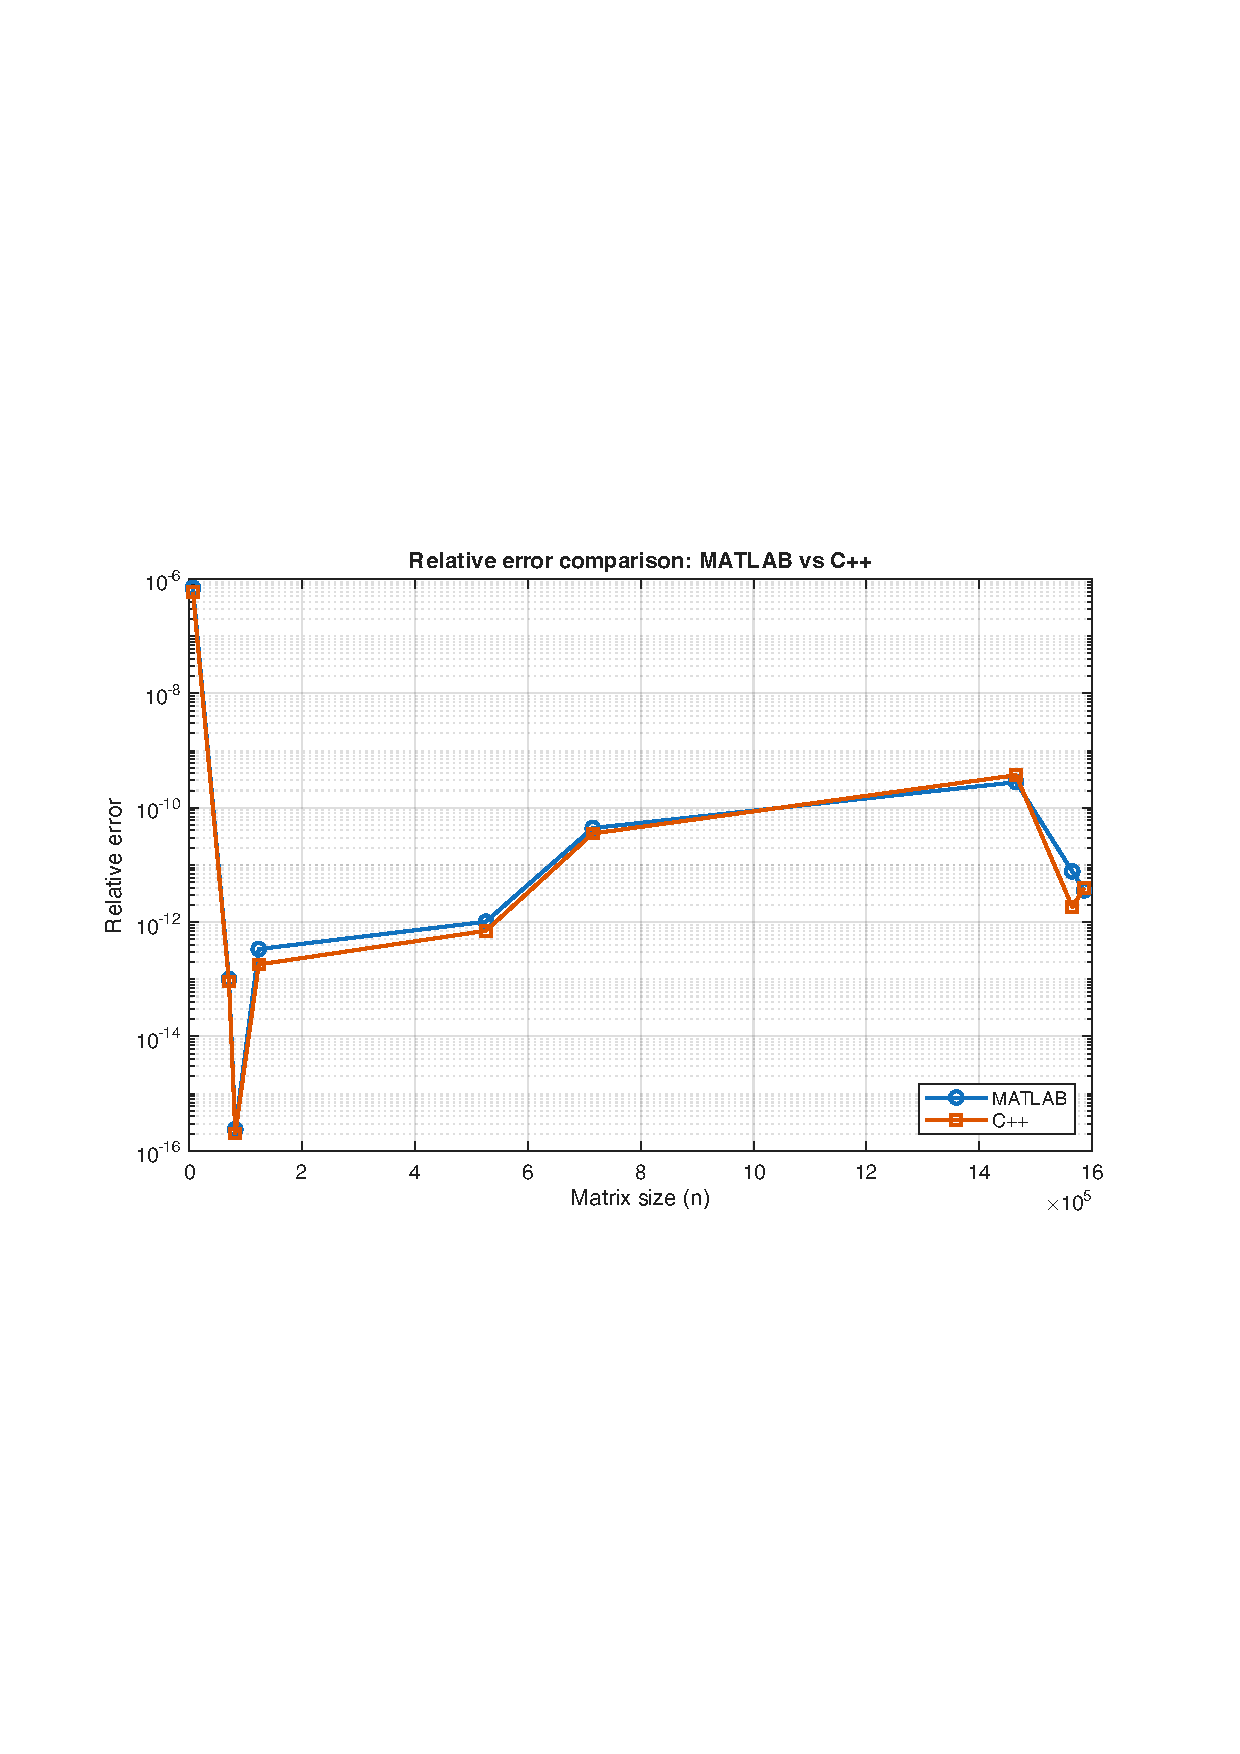
\includegraphics[
        width=\textwidth,
        trim= 0cm 9cm 0cm 9cm,
        clip
    ]{../plots/comparison/windows/relative_error_comparison.pdf}
    \caption{Confronto degli errori relativi su Windows}
    \label{fig:windows_relerr}
\end{figure}
\begin{figure}[hbt]
    \centering
    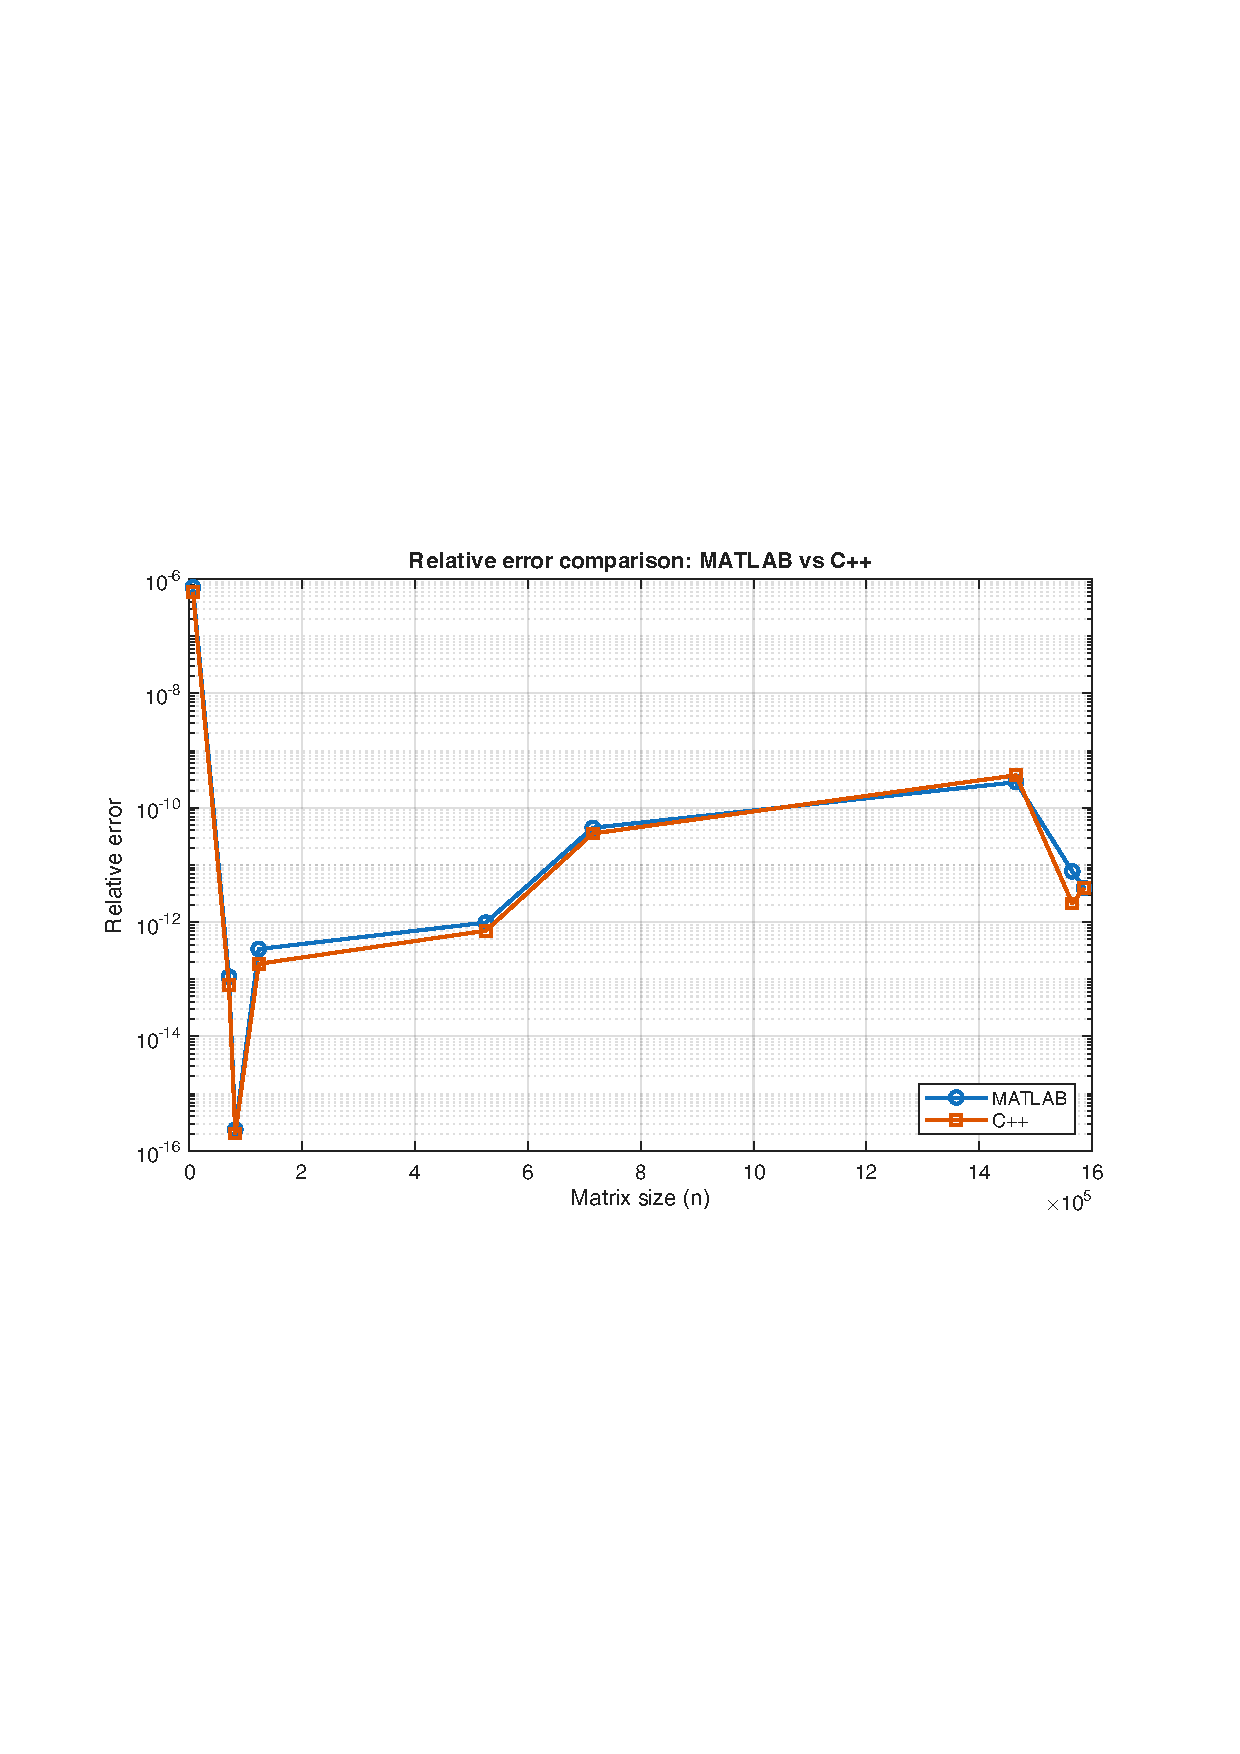
\includegraphics[
        width=\textwidth,
        trim= 0cm 9cm 0cm 9cm,
        clip
    ]{../plots/comparison/linux/relative_error_comparison.pdf}
    \caption{Confronto degli errori relativi su Linux}
    \label{fig:linux_relerr}
\end{figure}
\begin{figure}[H]
    \centering
    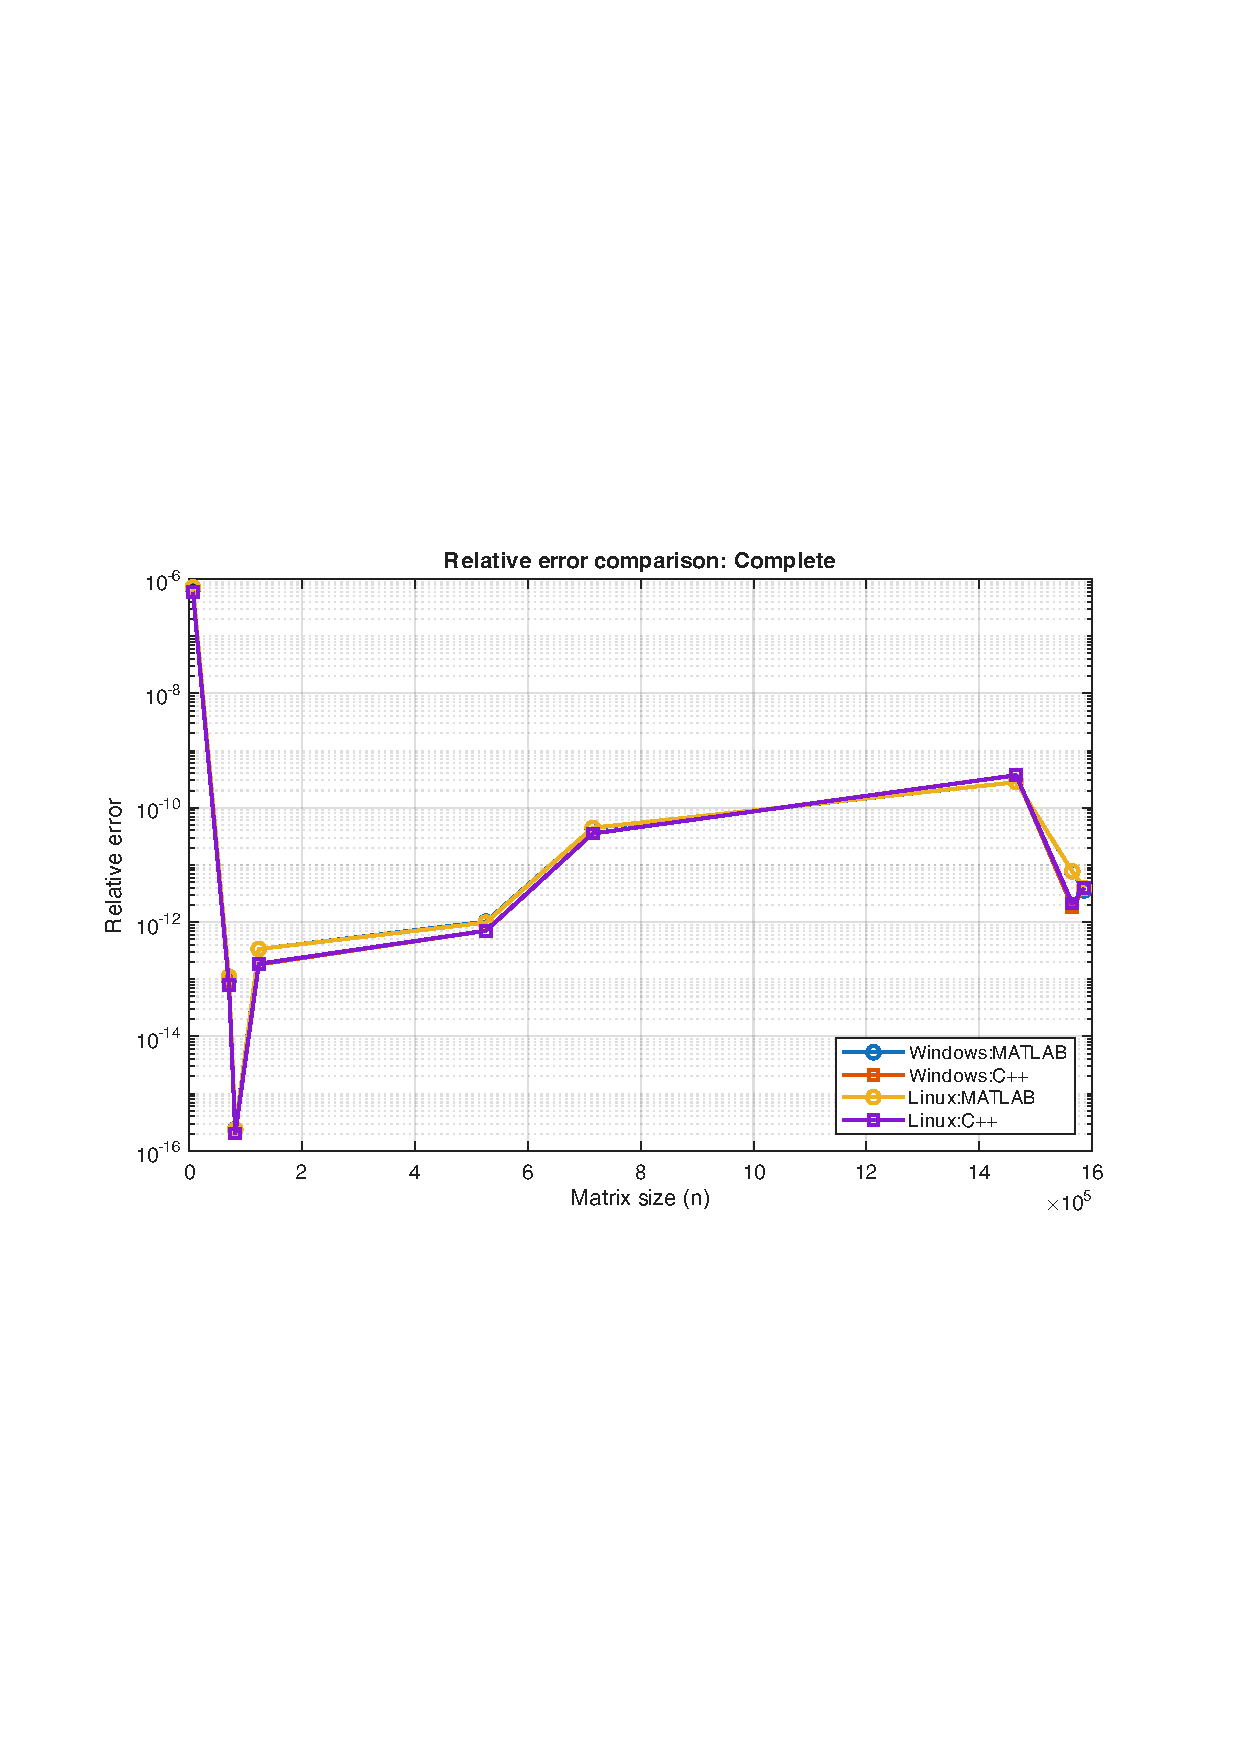
\includegraphics[
        width=\textwidth,
        trim= 0cm 9cm 0cm 9cm,
        clip
    ]{../plots/comparison/complete/relative_error_comparison.pdf}
    \caption{Confronto degli errori relativi su entrambi i sistemi operativi}
    \label{fig:complete_relerr}
\end{figure}